
\documentclass{eecslides}

% \usecolortheme{RimouskiDark}

\usepackage[frenchb]{babel}
\usepackage{lipsum}
\usepackage{graphicx}
\usepackage{caption}
\usepackage{hyperref}

\title[Les modèles]{\textbf{Les modèles:\\}Des outils indispensables pour biologiste 2.0}
\author[SV]{Steve Vissault}
\website{s.vissault@yahoo.fr}
\institute[Chaire de recherche EEC]{\textbf{Chaire de recherche en écologie des écosystèmes continentaux}}
\date{\today}

\begin{document}

	\begin{frame}[plain]
		\titlepage
	\end{frame}

	% \frame {
	%   \frametitle{Table des matières}
	%   \hspace{1cm}
	%   \parbox{0.9\textwidth}{
	%     \tableofcontents
	%   }
	% }

%%%%%%%%%%%%%%%%
	\section{Introduction}
%%%%%%%%%%%%%%%%
	\begin{frame}{Introduction}
	    		  
		    \begin{itemize}
			\item Introduction à la recherche (avec Dr. Gravel)
			\item Chaire de recherche du Canada en écologie des écosystèmes continentaux.
			\item \textbf{Sujet:} "Comment modéliser la réponde des peuplements aux changements climatiques ?"
		    \end{itemize}
		    
		\begin{figure}
			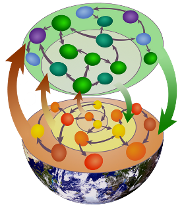
\includegraphics[width=0.2\linewidth]{logoCREEC.png}
			\caption*{\scriptsize \alert{\textbf{Logo EEC}}} 
		\end{figure}

	\end{frame}
%%%%%%%%%%%%%%%%
	\begin{frame}{Objectifs de la présentation}
	    		  
		    \begin{enumerate}
			\item Démystifier le concept de la modèlisation
			\item L'utilité et la pertinence de ses outils 
			\item La démarche d'un modélisateur
			\item Expliquer brièvement les grandes familles de modèles utilisées dans le contexte des changements climatiques
		    \end{enumerate}
	\end{frame}

%%%%%%%%%%%%%%%%
	\section{Mise en contexte}
%%%%%%%%%%%%%%%%

	\begin{frame}{Mise en contexte}{Analogie avec le Web 2.0} 

	\begin{itemize}
		\item Le \alert{web 2.0} est l'évolution d'internet vers davantage de simplicité (réseau sociaux, WordPress \dots)
		\item Rupture d'échelle qui mène à une utilisation plus large des \textit{"web services"}
	\end{itemize}

		\begin{figure}
			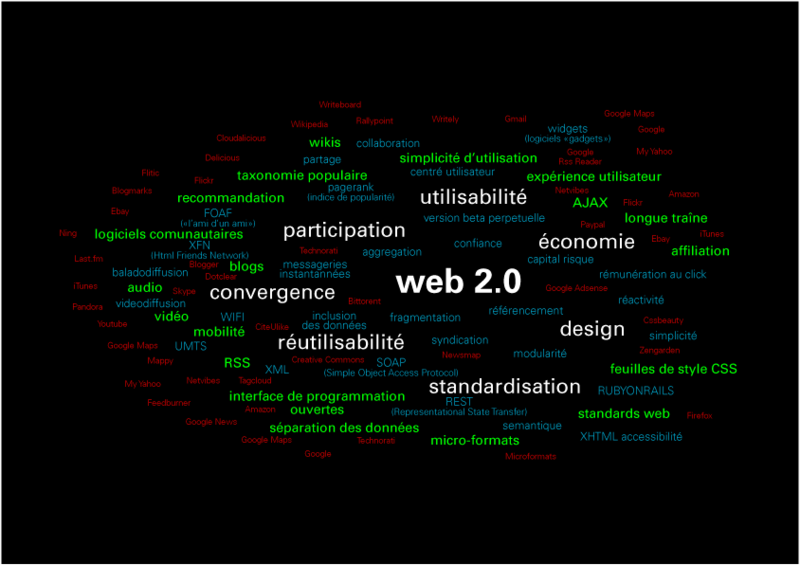
\includegraphics[width=0.5\textwidth]{800px-Carte_web_2.png}
	         		\caption*{\scriptsize\textbf{Source:}Wikipedia.org} 
		\end{figure}

	\end{frame}

%%%%%%%%%%%%%%%%
	\begin{frame}{Mise en contexte}{Définition d'un modèle}
	    
		\begin{itemize}
			\item Une simplification de la réalité
			\item Vise à comprendre et à prédire la dynamique complexe d'un système
		\end{itemize}

		% Historique de l'évolution des modèles
	
	\end{frame}

%%%%%%%%%%%%%%%%
	\begin{frame}{Mise en contexte}{Les approches conceptuelles} 
		
	
	\end{frame}

%%%%%%%%%%%%%%%%
	\section{Conclusion}
%%%%%%%%%%%%%%%%

	\begin{frame}{Conclusion}
	
	\begin{itemize}
		\item \textit{“Models are never true; fortunately it’s only necessary that they are useful.”} \textbf{Georges Box}
	\end{itemize}
	
	\end{frame}


	\begin{frame}[t]{Conclusion}{Remerciements} 
	\begin{center}
		Merci à \alert{Dominique Gravel} et à l'ensemble de \alert{mes collègues}

		\vspace{0.5cm}
		\Large{\textbf{\alert{Des questions?}}}
		
		\vspace{0.5cm}

		\small Présentation générée par \alert{$\LaTeX$} et disponible librement sur \href{https://github.com/SteveViss/Colloque_Models}{\alert{Github}}
	\end{center}

	\end{frame}

\end{document}